\documentclass[conference,a4paper]{IEEEtran}

\usepackage{amsmath,amssymb}
\usepackage{booktabs}
\usepackage{graphicx}
\usepackage{cite}
\usepackage{url}
\usepackage{siunitx}
\usepackage{tikz}
\usepackage{pgfplots}
\usetikzlibrary{arrows.meta,positioning}
\pgfplotsset{compat=1.18}

\title{Physics-Gated Reliable Adaptation of Phase-Coded FMCW ISAC for High-Mobility Vehicular Operation}

\author{\IEEEauthorblockN{Anonymous Author(s)}
\IEEEauthorblockA{Affiliation and contact information to be inserted before submission}}

% Compact RadarConf 2027 figures.

\newcommand{\radarconfArchitecture}{%
\begin{figure}[t]
\centering
\resizebox{\columnwidth}{!}{%
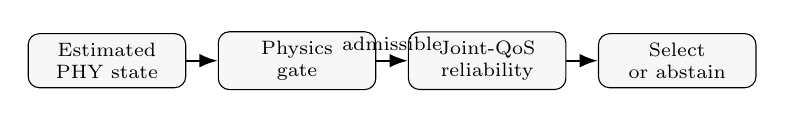
\begin{tikzpicture}[font=\scriptsize,node distance=4mm and 4mm,
box/.style={draw,rounded corners,align=center,minimum height=6.5mm,minimum width=20mm,fill=black!3},
arr/.style={-Latex,thick}]
\node[box] (state) {Estimated\\PHY state};
\node[box, right=of state] (gate) {Physics\\gate};
\node[box, right=of gate] (rel) {Joint-QoS\\reliability};
\node[box, right=of rel] (sel) {Select\\or abstain};
\draw[arr] (state) -- (gate);
\draw[arr] (gate) -- node[above]{admissible} (rel);
\draw[arr] (rel) -- (sel);
\end{tikzpicture}}
\caption{Admissibility-first control. Physically unsupported PC-FMCW actions are removed before uncertainty-aware joint sensing/communication qualification.}
\label{fig:radarconf-architecture}
\end{figure}}

\newcommand{\radarconfMainResults}{%
\begin{figure*}[t]
\centering
\begin{minipage}{0.49\textwidth}
\centering
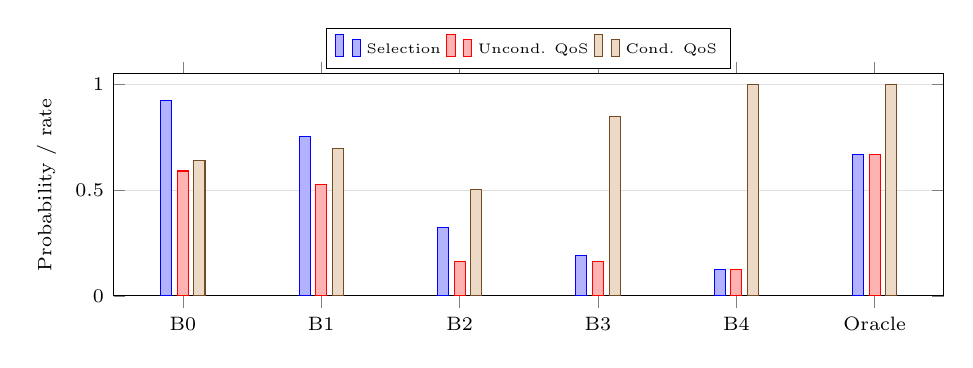
\begin{tikzpicture}
\begin{axis}[
width=\linewidth,height=4.4cm,
ybar,bar width=4pt,
ymin=0,ymax=1.05,
ylabel={Probability / rate},
symbolic x coords={B0,B1,B2,B3,B4,Oracle},xtick=data,
legend style={at={(0.5,1.02)},anchor=south,legend columns=3,font=\tiny},
tick label style={font=\scriptsize},label style={font=\scriptsize},
ymajorgrids=true,major grid style={black!12}]
\addplot coordinates {(B0,0.9235833)(B1,0.7531667)(B2,0.3225833)(B3,0.1906667)(B4,0.1223333)(Oracle,0.6666667)};
\addplot coordinates {(B0,0.5904167)(B1,0.5259167)(B2,0.16175)(B3,0.16175)(B4,0.1223333)(Oracle,0.6666667)};
\addplot coordinates {(B0,0.6392673)(B1,0.6982740)(B2,0.5014208)(B3,0.8483392)(B4,1.0)(Oracle,1.0)};
\legend{Selection,Uncond. QoS,Cond. QoS}
\end{axis}
\end{tikzpicture}
\end{minipage}\hfill
\begin{minipage}{0.49\textwidth}
\centering
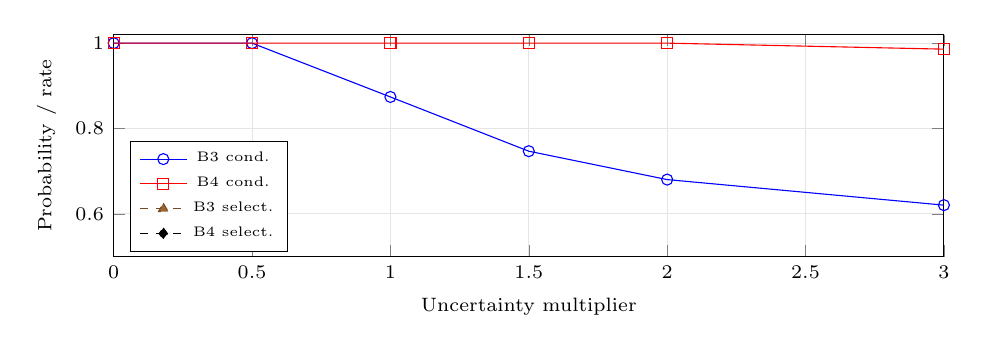
\begin{tikzpicture}
\begin{axis}[
width=\linewidth,height=4.4cm,
xlabel={Uncertainty multiplier},
ylabel={Probability / rate},
xmin=0,xmax=3,ymin=0.5,ymax=1.02,
legend style={font=\tiny,at={(0.02,0.02)},anchor=south west},
tick label style={font=\scriptsize},label style={font=\scriptsize},
grid=major,major grid style={black!10}]
\addplot+[mark=o] coordinates {(0,1)(0.5,1)(1,0.8739)(1.5,0.7468)(2,0.6803)(3,0.6204)};
\addplot+[mark=square] coordinates {(0,1)(0.5,1)(1,1)(1.5,1)(2,1)(3,0.9859)};
\addplot+[mark=triangle*,dashed] coordinates {(0,0.1667)(0.5,0.1667)(1,0.185)(1.5,0.1975)(2,0.2033)(3,0.2283)};
\addplot+[mark=diamond*,dashed] coordinates {(0,0.1667)(0.5,0.1617)(1,0.125)(1.5,0.1117)(2,0.0975)(3,0.0592)};
\legend{B3 cond.,B4 cond.,B3 select.,B4 select.}
\end{axis}
\end{tikzpicture}
\end{minipage}
\caption{Left: frozen paired benchmark over 12,000 state/seed units per policy. Right: increasing state uncertainty contracts B4's selected operating region while preserving higher conditional joint QoS until the strongest tested uncertainty setting.}
\label{fig:radarconf-results}
\end{figure*}}


\begin{document}
\maketitle

\begin{abstract}
High-mobility PC-FMCW ISAC must choose configurations that are not only attractive in QoS terms but physically capable of representing the requested range and velocity. We propose an admissibility-first controller for a \SI{77}{GHz} vehicular PC-FMCW PHY. Range, IF-sampling, and unambiguous-velocity constraints prune a 54-action space before uncertainty-aware joint sensing/communication qualification with a one-sided Wilson bound. The robust policy selects 12.23\% of cases with 100\% observed conditional joint QoS (99.816\% lower bound), versus 19.07\% selection and 84.83\% conditional QoS for deterministic joint adaptation. The resulting gain is a reliability--availability--computation trade-off, not universal policy dominance.
\end{abstract}

\begin{IEEEkeywords}
integrated sensing and communication, PC-FMCW, automotive radar, robust adaptation, high mobility, reliability, abstention
\end{IEEEkeywords}

\section{Introduction}

Phase-coded frequency-modulated continuous-wave (PC-FMCW) signaling can retain FMCW range--Doppler sensing while embedding communication information in the phase sequence. Automotive PC-FMCW and RadCom are already well established: prior work covers system design and interference mitigation \cite{uysal2020pcfmcw}, synchronization between automotive units \cite{lampel2020sync}, experimental joint sensing/communication \cite{kumbul2021experimental}, receiver architectures and waveform smoothing \cite{kumbul2022receiver,kumbul2022smoothed}, and sensing/communication performance trade-offs \cite{kumbul2023performance}. More recent FMCW ISAC work includes phase/index modulation, dynamic waveform reconfiguration, and hardware measurements \cite{temiz2026impm,temiz2026tcomm}. The open question addressed here is therefore not whether PC-FMCW can support both functions.

In high-mobility operation, two qualitatively different failure mechanisms arise. First, a waveform profile may be physically incapable of representing the requested state because the beat frequency exceeds the supported IF band or the radial velocity exceeds the unambiguous Doppler interval. Second, a physically valid action can still violate communication or sensing QoS because SNR, residual synchronization error, interference, and related PHY quantities are imperfectly known. Robust waveform and beamforming design under uncertainty is itself established \cite{wang2024robustwaveform,lyu2024dualrobust}, as is adaptive waveform selection in cognitive radar and ISAC \cite{tholeti2024online,yazar2026adaptive}. What remains comparatively underexplored is the ordering of these decisions for a finite PC-FMCW vehicular PHY.

We therefore study an \emph{admissibility-first} controller. Hard PC-FMCW capability limits are enforced before any stochastic ranking. Among the remaining actions, joint sensing/communication reliability is estimated under state uncertainty and accepted only when a finite-sample lower confidence bound reaches the target. If no action qualifies, the controller abstains. This separates physical infeasibility, statistical unreliability, and resource preference instead of collapsing them into a single optimization score.

\radarconfArchitecture

The contribution is threefold. First, we formulate a finite PC-FMCW adaptation problem in which range, IF-sampling, and unambiguous-velocity support are hard preconditions. Second, we couple the surviving actions to uncertainty-aware joint QoS qualification with an explicit reject option. Third, we show experimentally that robustness contracts the usable operating region: selected-case reliability increases, but availability and computation worsen. The principal result is thus an operating-region trade-off rather than a claim that the robust policy dominates every baseline.

\section{PC-FMCW Model and Physical Admissibility}

For chirp index $m$ and fast time $t$, the transmitted waveform is modeled as
\begin{equation}
s_m(t)=\sqrt{P_m}\exp\{j[\pi\mu t^2+\phi_m(t)]\},
\end{equation}
where $\mu=B/T_c$ is chirp slope and $\phi_m(t)$ carries the phase-coded communication sequence. For monostatic sensing, target range $R$ and radial velocity $v$ produce
\begin{equation}
\tau_r=\frac{2R}{c},\qquad f_{D,r}=\frac{2vf_c}{c},
\end{equation}
and after dechirping the reference beat frequency is $f_b=\mu\tau_r+f_{D,r}$. The remote communication path is one-way, with $\tau_c=R/c$ and $f_{D,c}=vf_c/c$.

The controller does not allow every waveform profile to compete at every operating point. For IF sample rate $F_s$, chirp repetition interval $T_r$, wavelength $\lambda$, and $N_c$ slow-time chirps, the relevant capability quantities include
\begin{align}
\Delta R &= \frac{c}{2B}, &
R_{\max}^{(+\mathrm{IF})} &= \frac{cF_s}{4\mu},\\
v_{\max} &= \frac{\lambda}{4T_r}, &
\Delta v &= \frac{\lambda}{2N_cT_r}.
\end{align}
An action is removed if the requested $(R,v)$ lies outside its physical support.

Two profiles are used. A source-grounded short-range profile at \SI{77}{GHz} uses an \SI{858}{MHz} valid sweep, \SI{10}{MSPS} IF sampling, and $T_r=\SI{115.8}{\micro s}$, yielding approximately 22.36~m positive-IF range support and 8.41~m/s unambiguous radial velocity \\cite{tiParking}. A composite high-mobility profile uses a \SI{1}{GHz} sweep, \SI{37.5}{MSPS} sampling, and $T_r=\SI{20}{\micro s}$, yielding approximately 56.21~m and 48.67~m/s. The latter is a capability reference rather than a claimed commercial preset.

The frozen action space combines two profiles, chip budgets $\{16,32,64\}$, transmit-power backoffs $\{0,3,6\}$~dB, and repetition factors $\{1,2,4\}$:
\begin{equation}
|\mathcal A|=2\times3\times3\times3=54.
\end{equation}
These variables are kept explicit because they change physical support, communication rate, SNR, and repetition overhead in interpretable ways.

\section{Reliability-Constrained Selection}

Let $S$ denote the uncertain PHY state, including communication and sensing SNR, range, velocity, residual CFO/synchronization error, interference, and phase-noise state. The physical gate produces $\mathcal A_{\rm phys}(\hat S)\subseteq\mathcal A$. For each admissible action, uncertainty samples are drawn around the estimated state and the binary event
\begin{align}
\mathcal E=\{&
\mathrm{BER}\le10^{-3},\;
R_{\rm eff}\ge\SI{100}{kbps}, \nonumber\\
&\mathrm{RMSE}_R\le\SI{1}{m},\;
\mathrm{RMSE}_v\le\SI{1}{m/s}\}.
\end{align}
is evaluated.

If $k$ of $N$ uncertainty draws satisfy $\mathcal E$, the empirical fraction $\hat p=k/N$ is not treated as a certificate. We instead use the one-sided Wilson lower bound \cite{brown2001binomial}
\begin{equation}
L_W=
\frac{\hat p+\frac{z^2}{2N}
-z\sqrt{\frac{\hat p(1-\hat p)}{N}+\frac{z^2}{4N^2}}}
{1+\frac{z^2}{N}},
\end{equation}
with $z=\Phi^{-1}(0.95)$. B4 admits an action only when $L_W\ge0.95$, then selects the lowest declared resource-cost action among those admitted. If no action qualifies, it abstains.

This rule makes the draw budget part of the controller. With all trials successful, $L_W=N/(N+z^2)$; hence 32/32 successes can reach only about 0.922, so a 0.95 target is structurally unattainable with 32 draws. The frozen controller uses 512 internal draws. The 4096-draw supplemental comparator is used only to assess Monte-Carlo decision stability; it is not physical ground truth.

We compare six policies on common states: a fixed policy B0; communication-only B1; sensing-only B2; deterministic joint B3, which treats the estimate as exact; robust joint B4; and a non-deployable hindsight Oracle. The Oracle uses receiver-level truth and is only a reference.

\section{Evaluation}

The frozen benchmark uses 12 predeclared scenarios and 1000 common seeds, yielding 12,000 state/seed units per policy and 72,000 final receiver evaluations across six policies. Each final communication evaluation uses 20,000 bits, and sensing error is evaluated with repeated noisy IF trials. Policy differences are paired on the same state/seed bank; reported paired intervals use 10,000 bootstrap resamples.

The study also includes uncertainty scaling, gate and constraint ablations, model-mismatch tests, finite-draw calibration, resource analysis, and host-runtime measurements. All numerical evidence is simulation, analytical, statistical, or host-runtime output; no adaptive-controller hardware measurement is claimed.

\radarconfMainResults

\section{Results}

\subsection{Robustness trades availability for selected-case reliability}

Figure~\ref{fig:radarconf-results} summarizes the main result. B3 selects in 19.07\% of evaluated cases and attains 84.83\% conditional joint QoS. B4 selects only 12.23\%, but all 1,468 selected cases satisfy the joint event, corresponding to a one-sided 95\% Wilson lower bound of 99.816\%. This stronger selected-case evidence is purchased by 87.77\% abstention.

Consequently, B4 does \emph{not} maximize unconditional joint QoS. Its unconditional probability is 12.23\%, compared with 16.18\% for B3. The paired B4--B3 difference is $-0.03942$ with a 95\% bootstrap interval $[-0.04292,-0.03600]$. The robust policy is therefore a conservative operating-region selector, not a universally superior controller.

The uncertainty sweep supports the same interpretation. At zero uncertainty, B3 and B4 coincide at 16.67\% selection and 100\% conditional QoS. At uncertainty scale two, B3 selects 20.33\% with 68.03\% conditional QoS, while B4 contracts to 9.75\% selection and retains 100\% observed conditional QoS. At scale three, B4 selects only 5.92\%; its observed success fraction is 98.59\%, but the one-sided Wilson lower bound falls to 93.93\%, below the target. Robustness therefore contracts rather than indefinitely protects the operating region.

\subsection{The physical gate and confidence rule are consequential}

Ablations separate hard infeasibility from ordinary robustness. On the supplemental bank, FULL\_B4 selects 12.50\% with 100\% observed conditional joint QoS. Removing state uncertainty expands selection to 20.00\% but lowers conditional joint QoS to 80.83\%. Removing the joint constraint expands selection to 67.25\% with 85.50\% conditional joint QoS.

Removing the physics gate is more severe: the evaluated ungated variant selects 31.67\% of states but obtains 0\% joint QoS. This result is specific to the frozen action set and does not imply that every ungated optimizer must fail; it shows that physically unsupported profiles can corrupt the ranking if they are allowed to compete with admissible actions.

Finite-draw calibration gives the computational side of the trade-off. Relative to the nested 4096-draw comparator, feasibility-decision disagreement decreases from 0.583\% at 64 draws to 0\% at 512 draws, while selected-action disagreement remains 0.833\% at 512 draws. On the unoptimized Python/Linux host, B4 median decision time rises from 32.17~ms at 64 draws to 251.04~ms at 512 draws; the 512-draw 95th percentile is 504.11~ms. These timings are not embedded-ECU claims.

\radarconfEvidenceTable

\subsection{Mismatch exposes the limit of robustness}

B4 remains useful under several moderate mismatches in the tested banks. With residual CFO larger than assumed, or actual radial speed above the nominal Doppler condition, B4 preserves higher joint QoS than B3. Under interference under-modeling from assumed INR $-10$~dB to actual 0~dB, B4 reaches 86\% joint QoS while B3 falls to 18\%. However, at actual INR of 10--20~dB both policies fail; when the controller assumes 12~dB SNR but the actual value is 8~dB, B4 falls to 17\%, and at 6~dB both fail. The reliability claim is therefore conditional on the uncertainty model representing the operating error with reasonable fidelity.

\section{Discussion and Conclusion}

Recent PC-FMCW and FMCW-ISAC literature already demonstrates waveform feasibility, synchronization, receiver processing, dynamic reconfiguration, and hardware implementations \cite{alamieldine2024chirpseq,alamieldine2026sync,temiz2026tcomm}. Robust ISAC design and adaptive waveform selection are likewise established \cite{wang2024robustwaveform,yazar2026adaptive}. The contribution here is narrower: the controller makes physical admissibility a precondition for stochastic reliability qualification and is allowed to reject states that cannot be supported with the declared evidence.

The experiments show why this distinction matters. A robust policy can improve the reliability of the states it serves while simultaneously reducing total service availability. Increasing the Monte-Carlo budget stabilizes the decision but raises latency. Severe mismatch can remove the reliable region altogether. These observations argue against reporting a single success rate for adaptive ISAC; physical infeasibility, abstention, conditional reliability, unconditional service probability, and computational cost should be reported separately.

The present work is limited to simulation and host-runtime evidence. The communication receiver is a transparent DBPSK reference rather than a measured automotive communication standard, the high-mobility profile is a composite capability reference, and the current B4 implementation is not real-time. Hardware-in-the-loop validation, higher-fidelity oscillator/channel models, faster confidence tests, and larger action spaces are natural next steps.

Within those limits, the result is clear: physics-gated robust PC-FMCW adaptation identifies a smaller but better-supported operating region under high-mobility uncertainty. The scientific outcome is not unconditional dominance; it is an explicit reliability--availability--computation boundary.

\bibliographystyle{IEEEtran}
\bibliography{references_v2_1,references_submission}

\end{document}
